\documentclass{article}
\newsavebox{\oldepsilon}
\savebox{\oldepsilon}{\ensuremath{\epsilon}}
\usepackage[minionint,mathlf,textlf]{MinionPro} % To gussy up a bit
\renewcommand*{\epsilon}{\usebox{\oldepsilon}}
\usepackage[margin=1in]{geometry}
\usepackage{graphicx} % For .eps inclusion
%\usepackage{indentfirst} % Controls indentation
\usepackage[compact]{titlesec} % For regulating spacing before section titles
\usepackage{adjustbox} % For vertically-aligned side-by-side minipages
\usepackage{array, amsmath,  mhchem}
\usepackage[hidelinks]{hyperref}
\usepackage{courier, subcaption}
\usepackage{multirow, enumerate}
\usepackage[autolinebreaks,framed,numbered]{mcode}
\usepackage{float}
\restylefloat{table}

\pagenumbering{gobble} 
\setlength\parindent{0 cm}
\renewcommand{\arraystretch}{1.2}
\begin{document}
\large

MCB 135 Problem Set 7 \hfill Due Wednesday, April 1, 2015 at 2:30 PM

\section*{Problem 1: Noise-induced oscillations (Ingalls 7.8.27, 45 points)}

Stochastic systems can exhibit a range of oscillatory behaviors, ranging from near-perfect periodicity to erratic cycles. To explore this behavior, consider a stochastic relaxation oscillator studied by Jos\'{e} Vilar and colleagues (Vilar et al., 2002). The system involves an activator and a repressor. The activator enhances expression of both proteins. The repressor acts by binding the activator, forming an inert complex. A simple model of the system is:

\begin{eqnarray*}
\textrm{ Name and description } \hspace{2 cm} & \textrm{Reaction} & \hspace{2 cm} \textrm{Reaction propensity}\\ \hline
R_1 \textrm{ (activator synthesis) } \hspace{2 cm} & \ce{\varnothing {\color{white}.} -> b_A A} & \hspace{2 cm} \frac{\gamma_A}{b_A} \cdot \frac{\alpha_0 + N_A/K_A}{1 + N_A/K_A}\\
R_2 \textrm{ (repressor synthesis) } \hspace{2 cm} & \ce{\varnothing {\color{white}.} -> b_R R} & \hspace{2 cm} \frac{\gamma_R}{b_R} \cdot \frac{N_A/K_R}{1 + N_A/K_R}\\
R_3 \textrm{ (activator decay) } \hspace{2 cm} & \ce{A -> \varnothing} & \hspace{2 cm} \delta_A N_A \\
R_4 \textrm{ (repressor decay) } \hspace{2 cm} & \ce{R -> \varnothing} & \hspace{2 cm} \delta_R N_R \\
R_5 \textrm{ (association) } \hspace{2 cm} & \ce{A + R -> C} & \hspace{2 cm} k_C N_A N_R \\
R_6 \textrm{ (dissociation w/ activator decay) } \hspace{2 cm} & \ce{C -> R} & \hspace{2 cm} \delta_A N_C \\
\end{eqnarray*}

Here, $N_A$, $N_R$, and $N_C$ are the molecular counts for the activator, repressor, and activator-repressor complex. The parameters $b_A$ and $b_R$ characterize the expression burst size. The Hill-type propensities of the synthesis reactions are not well-justified at the molecular level, but these expressions nevertheless provide a simple formulation of a stochastic relaxation oscillator.

\begin{enumerate}[a)]
\item Take parameter values $\gamma_A = 250$, $b_A = 5$, $K_A = 0.5$, $\alpha_0 = 0.1$, $\delta_A = 1$, $\gamma_R = 50$, $b_R = 10$, $K_R=1$, $k_C = 200$, and $\delta_R = 0.1$. Run a Gillespie SSA simulation of this model and verify its quasi-periodic behavior.\\

\begin{lstlisting}
function [] = problem1a()
    gamma_A = 250; b_A = 5; K_A = 0.5; alpha_0 = 0.1; delta_A = 1;
    gamma_R = 50; b_R = 10; K_R = 1; k_C = 200; delta_R = 0.1;
    i = 1; n = 10000;
    a = zeros(1,n); a(1) = 0;
    r = zeros(1,n); r(1) = 0;
    c = zeros(1,n); c(1) = 0;
    t = zeros(1,n); t(1) = 0;
    
    while i < n
        rates = [ (gamma_A/b_A) * (alpha_0 + a(i)/K_A)/(1 + a(i)/K_A), ...
            (gamma_R/b_R) * (a(i)/K_R)/(1 + a(i)/K_R), ...
            delta_A*a(i), ...
            delta_R*r(i), ...
            k_C * a(i) * r(i), ...
            delta_A * c(i) ];
        t(i+1) = t(i)+exprnd(1/sum(rates));
        event = randsample(6,1,true, rates ./ sum(rates));
        if event == 1
            a(i+1) = a(i) + b_A; r(i+1) = r(i); c(i+1) = c(i);
        elseif event == 2
            a(i+1) = a(i); r(i+1) = r(i) + b_R; c(i+1) = c(i);
        elseif event == 3
            a(i+1) = a(i) - 1; r(i+1) = r(i); c(i+1) = c(i);
        elseif event == 4
            a(i+1) = a(i); r(i+1) = r(i) - 1; c(i+1) = c(i);
        elseif event == 5
            a(i+1) = a(i) - 1; r(i+1) = r(i) - 1; c(i+1) = c(i) + 1;
        elseif event == 6
            a(i+1) = a(i); r(i+1) = r(i) + 1; c(i+1) = c(i) - 1;
        end
        i = i + 1;
    end
    
    % Next calculate the probability distribution at the end
    plot(t,a,'b', 'LineWidth', 2); hold on;
    plot(t,r,'r', 'LineWidth', 2);
    plot(t,c,'k', 'LineWidth', 2);
    title('Stochastic simulation')
    xlabel('Time')
    ylabel('Molecule count')
    legend('A(t)', 'R(t)', 'C(t)', 'Location', 'NorthEast')
    set(gca,'FontSize',14)
    axis([100 250 0 max([a, r, c])])
    
end
\end{lstlisting}

\begin{center}
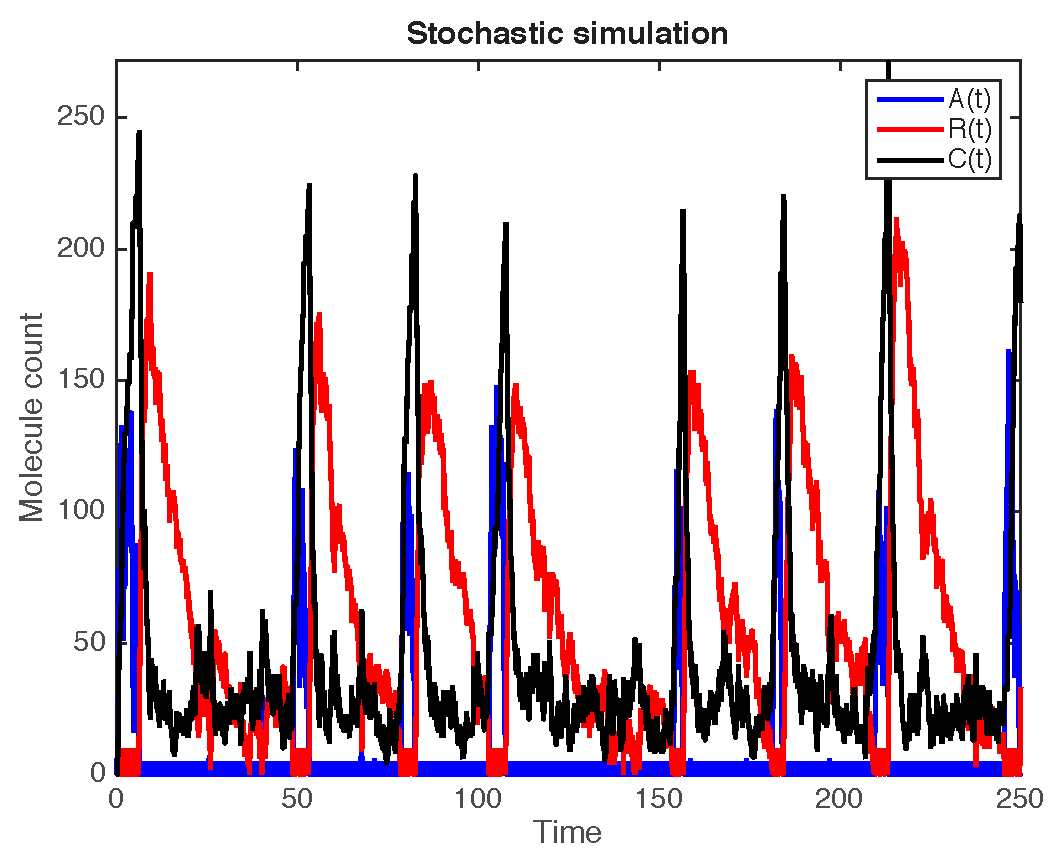
\includegraphics[width=0.6\textwidth]{prob1a.pdf}
\end{center}

\item The deterministic version of this model is:
\begin{eqnarray*}
\frac{da}{dt} = \gamma_A \frac{\alpha_0 + a/K_A}{1 + a/K_A} - k_C a r - \delta_A a\\
\frac{dr}{dt} = \gamma_R \frac{a/K_R}{1 + a/K_R} - k_C a r + \delta_A c - \delta_R r\\
\frac{dc}{dt} =  k_C a r - \delta_A c
\end{eqnarray*}
where $a$, $r$, and $c$ are the concentrations of activator, repressor, and complex. Run a simulation with the same parameter values as in part (a). Does the system exhibit oscillations? How is the behavior different if you set $\delta_R=0.2$?\\

\begin{lstlisting}
function [] = problem1b2()
    global gamma_A b_A K_A alpha_0 delta_A gamma_R b_R K_R k_C delta_R
    gamma_A = 250; b_A = 5; K_A = 0.5; alpha_0 = 0.1; delta_A = 1;
    gamma_R = 50; b_R = 10; K_R = 1; k_C = 200; delta_R = 0.2; % or delta_R = 0.1
    
    initial_concentrations = [5, 10, 35];
    time_interval = [0, 250];
    [timepoints, concentrations] = ode45(@chain1ddt, ...
        time_interval, initial_concentrations);
    
    % Next calculate the probability distribution at the end
    plot(timepoints, concentrations(:,1), '-b', 'LineWidth', 3); hold on;
    plot(timepoints, concentrations(:,2), '-r', 'LineWidth', 3);
    plot(timepoints, concentrations(:,3), '-k', 'LineWidth', 3);
    title('Deterministic simulation (\delta_R = 0.2)')
    xlabel('Time')
    ylabel('Molecule count')
    legend('A(t)', 'R(t)', 'C(t)', 'Location', 'NorthEast')
    set(gca,'FontSize',14)
    axis([0 250 0 max(max(concentrations))])
    
end

function changes_in_concentrations = chain1ddt(time, current_concentrations)
    global gamma_A b_A K_A alpha_0 delta_A gamma_R b_R K_R k_C delta_R

    A = current_concentrations(1);
    R = current_concentrations(2);
    C = current_concentrations(3);
   
    change_in_A = gamma_A*(alpha_0 + A/K_A)/(1+A/K_A) - k_C*A*R - delta_A*A;
    change_in_R = gamma_R*(A/K_R)/(1+A/K_R) - k_C*A*R + delta_A*C - delta_R*R;
    change_in_C = k_C*A*R - delta_A*C;
    
    changes_in_concentrations = [change_in_A; change_in_R; change_in_C];
end

\end{lstlisting}

{\color{red}
The system does not exhibit oscillations when $\delta_R=0.1$ (left figure). However, when $\delta_R=0.2$, oscillations are restored (right figure).
}

\begin{center}
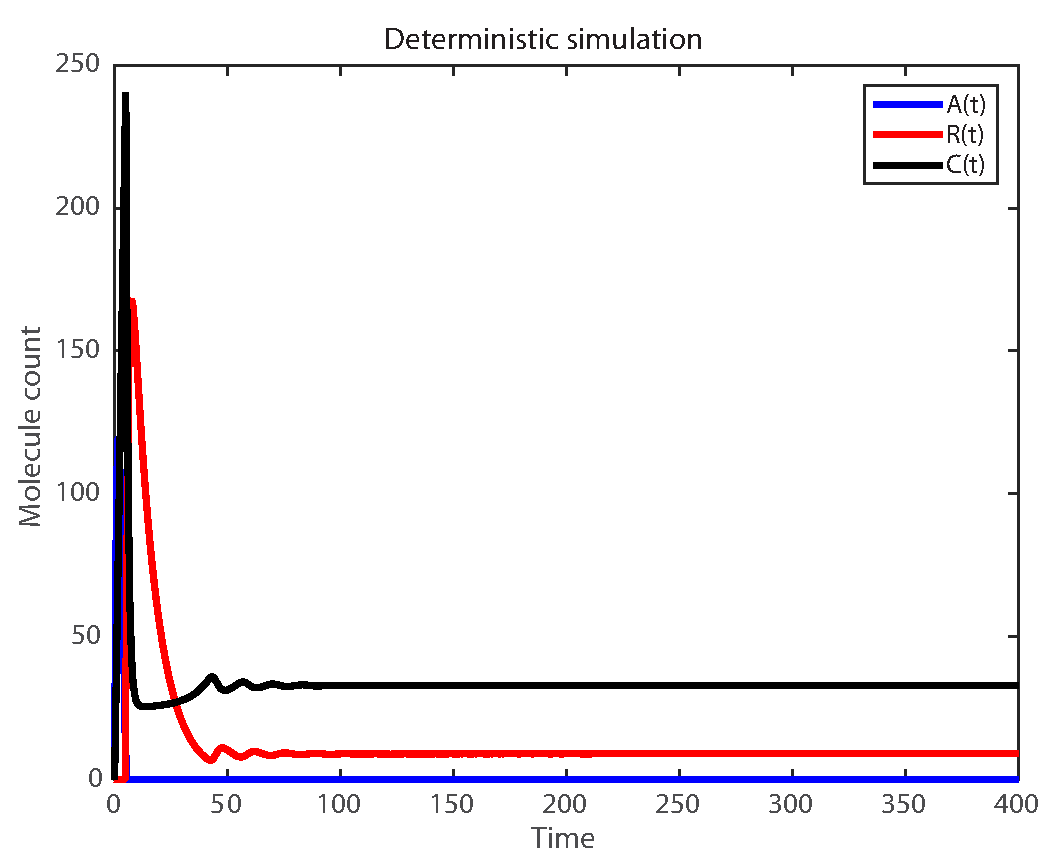
\includegraphics[width=0.4\textwidth]{prob1b.pdf} \hfill 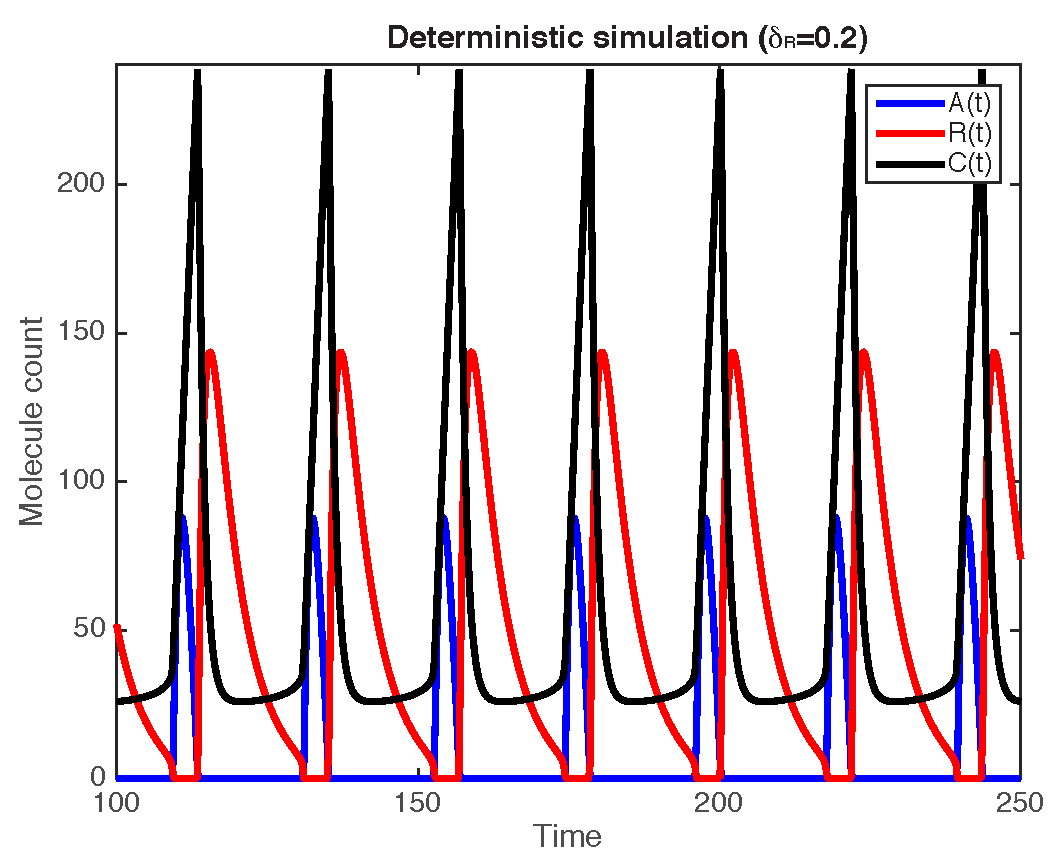
\includegraphics[width=0.4\textwidth]{prob1b2.pdf}
\end{center}

\item The contrast between the behavior of the models in parts (a) and (b), for $\delta_R=0.1$, can be explained by the excitability of this relaxation oscillato. Run two simulations of the deterministic model ($\delta_R=0.1$), one from initial conditions $(a,r,c)=(0,10,35)$ and another from initial conditions $(a,r,c)=(5,10,35)$. Verify that in the first case, the activator is quenched by the repressor, and the system remains at a low-activator steady state, whereas in the second case, this small quantity of activator is able to break free from the repressor and invoke a (single) spike in expression. Explain how noise in the activator abundance could cause repeated excitations by allowing the activator abundance to regularly cross the threshold. This is referred to as \textit{noise-induced oscillation}.\\

\begin{center}
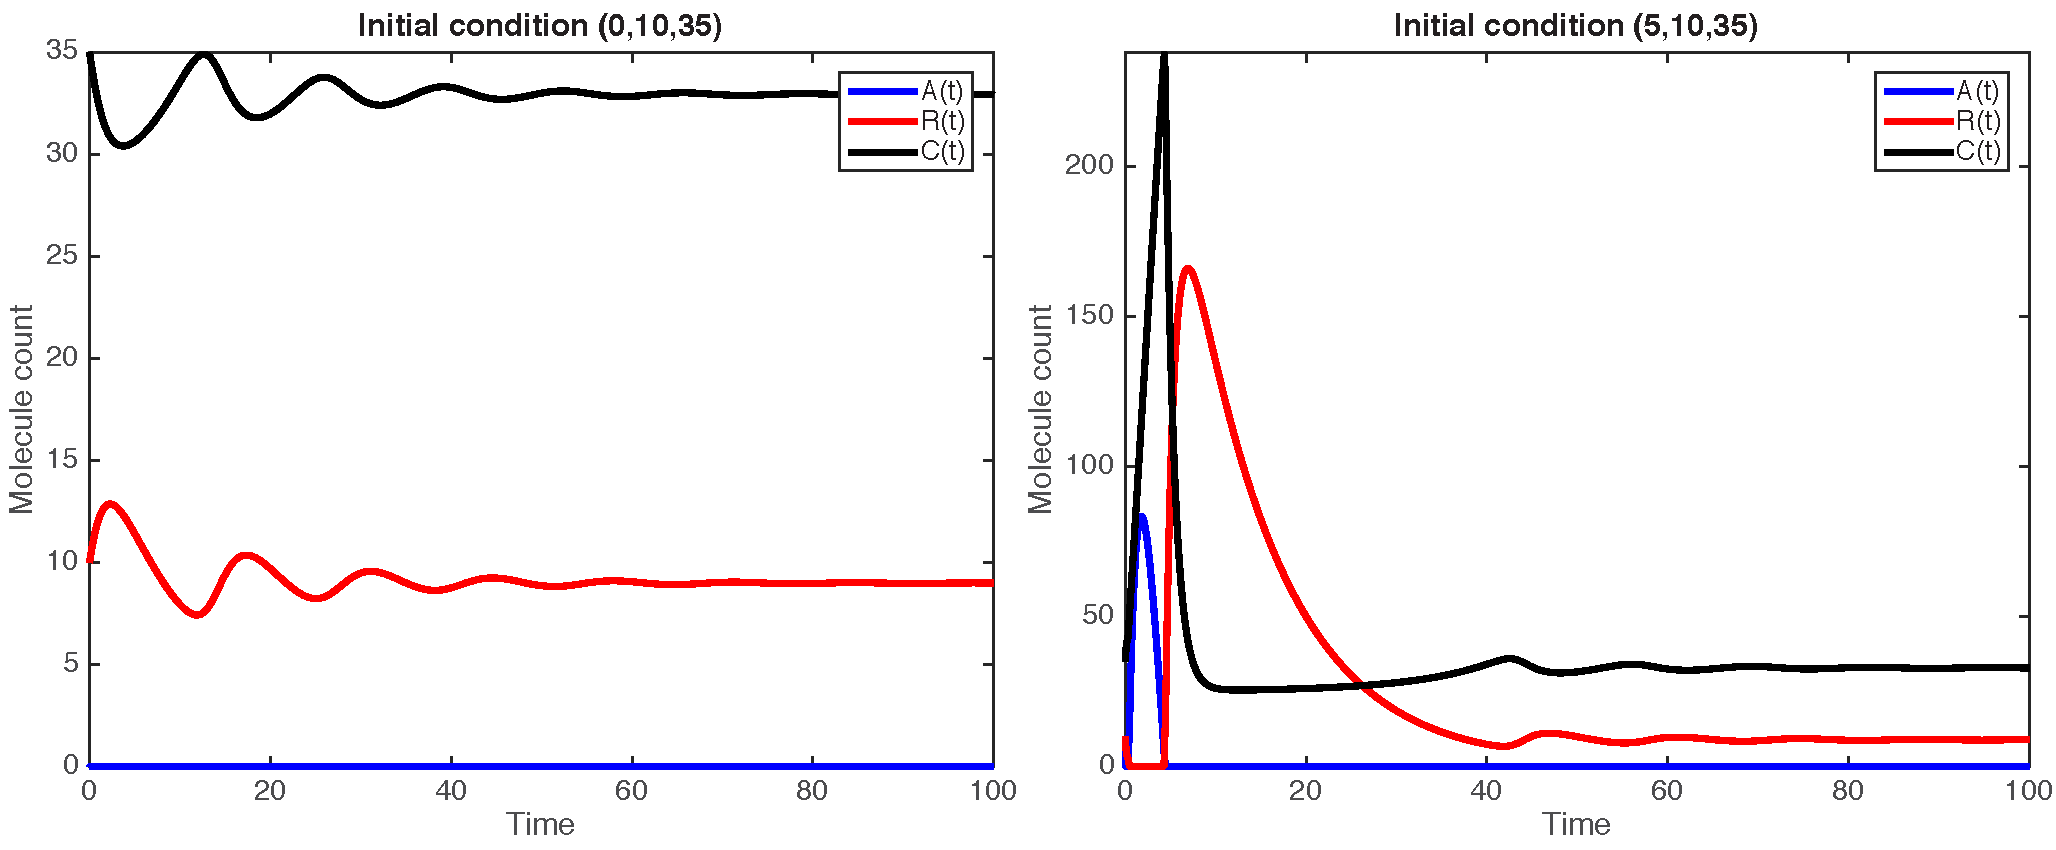
\includegraphics[width=0.9\textwidth]{prob1c.pdf}
\end{center}

{\color{red}
Code is a straightforward modification of the above. The ``burstiness" of expression could easily cause the activator to exceed its threshold abundance of $\leq$5, particularly since the bust size $b_A = 5$. (Even without bursting, $A$ will sometimes cross the activity threshold due to chance.)

}

\end{enumerate}

\section*{Problem 2: Effect of autorepression (55 points)}

Consider the open system
\[ \ce{\varnothing {\color{white} .} ->[k_1] A ->[k_2] \varnothing} \]
\begin{enumerate}[a)]
\item Find the master equation for this system.\\

{\color{red}
The trick to this problem is to recognize that the rate of the degradation reaction $\sim nk_2$ while the rate of the synthesis reaction is constant:
\[ \frac{dP(n,t)}{dt} = \left\{
     \begin{array}{lr}
       k_2 P(1,t) - k_1 P(0,t) & : n=0\\
       \left[n+1\right] k_2 P(n+1,t) + k_1 P(n-1,t) - \left[ k_1 + n k_2 \right] P(n,t) & : n>0
     \end{array}
   \right. \]

}

\item Show that, at steady state,
\[ P(N_A = n) = \frac{k_1}{k_2 n} P(N_A = n-1, t) \]
{\color{red}
We will show this by induction. For the base case:
\[ \frac{dP(0,t)}{dt} = 0 \implies P(1,t) = \frac{k_1}{k_2} P(0,t) \]
Now suppose that the stated formula is true for some value $x$, i.e. $P(x,t) = \frac{k_1}{k_2 x} P(x-1,t)$. We will show that the formula holds for $x+1$:
\begin{eqnarray*}
 \frac{dP(x,t)}{dt} = 0 \implies P(x+1,t) & = & \frac{1}{k_2(x+1)} \left[ - k_1 P(x-1,t) + \left( k_1 + x k_2 \right) P(x,t) \right]\\
 & = & \frac{1}{k_2(x+1)} \left[ - k_2 x P(x,t) + \left( k_1 + x k_2 \right) P(x,t)  \right]\\
 & = & \frac{k_1}{k_2(x+1)} P(x,t)
\end{eqnarray*}
Thus the stated formula applies for all $n \geq 0$. As the probability distribution does not depend on time at steady state, the argument $t$ can be omitted.
}

\item Use the Taylor series for $e^x$ to derive the steady-state probability distribution:
\[ P(N_A = n) = \frac{\left( \frac{k_1}{k_2} \right)^n e^{-k_1/k_2}}{n!} \]
{\color{red}
 Express our result from part (b) in terms of $P(0)$:
 \begin{eqnarray*}
P(n) = \frac{k_1}{k_2 n} P(n-1) = \frac{\left( \frac{k_1}{k_2} \right)^2}{n(n-1)} P(n-2) = \frac{\left( \frac{k_1}{k_2} \right)^n}{n!} P(0)
 \end{eqnarray*}
We can find $P(0)$ using the fact that the probabilities must sum to one:
\begin{eqnarray*}
 1 & = & P(0)\left[ 1 + \frac{k_1}{k_2} + \frac{k_1^2}{2k_2^2} + \ldots \right]\\
 & = & P(0) \sum_{i=0}^{\infty} \frac{\left( \frac{k_1}{k_2} \right)^i}{i!} = e^{k_1/k_2} P(0) \implies P(0) = e^{-k_1/k_2}
 \end{eqnarray*}
Plugging this into our result above, we obtain the desired expression:
 \[ P(n) = \frac{\left( \frac{k_1}{k_2} \right)^n e^{-k_1/k_2}}{n!} \]
 Note that this is just a Poisson distribution with parameter $\lambda=k_1/k_2$.
}

\item Perform a Gillespie SSA simulation of the open system above with $k_1=10, k_2=1$. Estimate the probability distribution $P(n)$ from the timecourse $A(t)$. (Exercise your judgment in ignoring data early in the simulation and choosing an appropriate timescale for the simulation.) Plot the Poisson probability density function with $\lambda=k_1/k_2$ on the same axes for comparison.\\

\begin{lstlisting}
function [] = problem1d()
    k1 = 10; k2 = 1;
    i = 1; n = 100000;
    a = zeros(1,n); a(1) = 10;
    t = zeros(1,n); t(1) = 0;
    
    while i < n
        rates = [k1, a(i)*k2];
        t(i+1) = t(i)+exprnd(1/sum(rates));
        event = randsample(2,1,true, rates ./ sum(rates));
        if event == 1
            a(i+1) = a(i) + 1;
        elseif event == 2
            a(i+1) = a(i) - 1;
        end
        i = i + 1;
    end
    
    bins = 0:1:max(a);
    a_binned = histc(a(n),bins)./n;
    disp(sprintf('%d %d',length(bins),length(a_binned)));
    plot(bins, a_binned, 'r', 'LineWidth', 2); hold on;
    plot(bins,poisspdf(bins,k1/k2),'k', 'LineWidth', 2)
    title('Simple regulation')
    xlabel('Molecules of A')
    ylabel('Probability')
    legend('Simulation', 'Theory','Location', 'NorthEast')
    set(gca,'FontSize',14)
    
end
\end{lstlisting}

\begin{center}
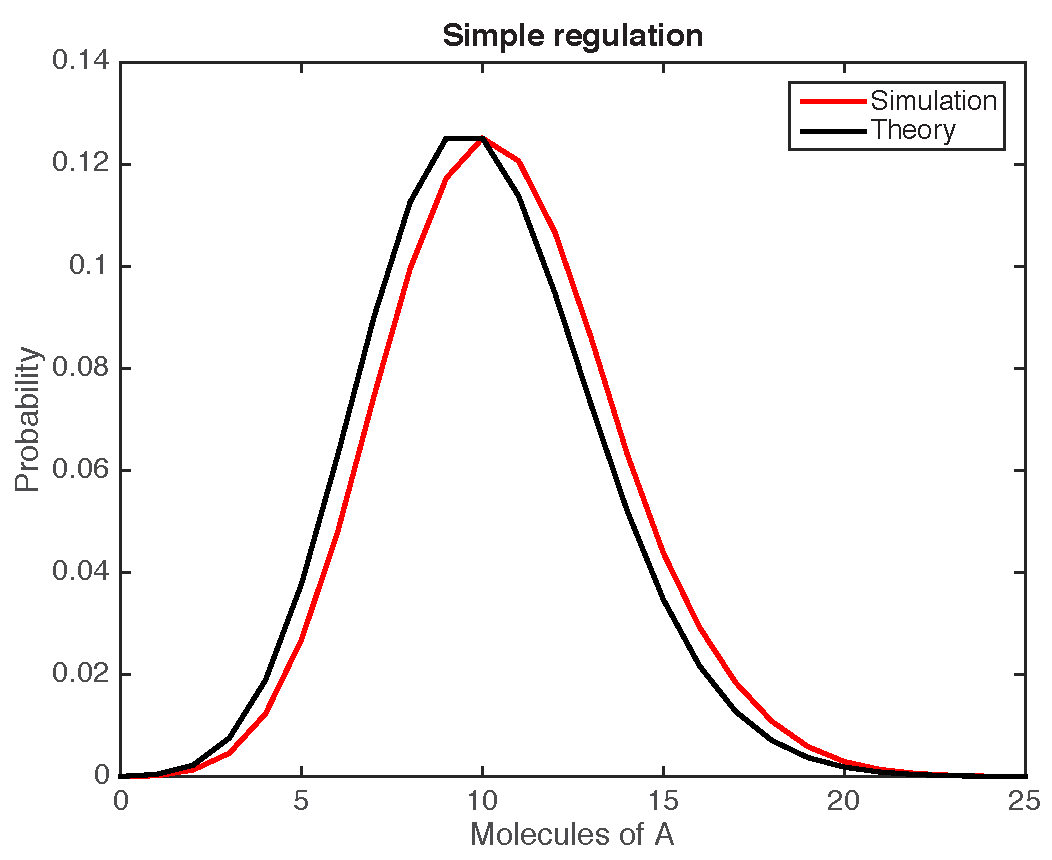
\includegraphics[width=0.4\textwidth]{prob1d.pdf}
\end{center}

{\color{red}
TODO: Figure out if there is a \mcode{histc()} issue.
}

\end{enumerate}
Now consider a related molecule that exhibits hyperbolic autorepression, i.e.
\[ \ce{\varnothing {\color{white} .} ->[k_1/(1+k_3B)] B ->[k_2] \varnothing} \]
\begin{enumerate}[a)]
\setcounter{enumi}{4}
\item Perform a Gillespie SSA simulation of this system with $k_1=100, k_2=k_3=1$ and estimate the probability distribution $P(n)$ from the timecourse $B(t)$. Fit a Poisson distribution to $P(n)$ and plot both on the same axes (e.g. using \mcode{poissfit()} and \mcode{poisspdf()} in MATLAB). Does the negative autoregulation system have more or less variance than expected for the simple regulation system?

\begin{lstlisting}
function [] = problem1e()
    k1 = 100; k2 = 1; k3 = 1;
    i = 1; n = 100000;
    b = zeros(1,n); b(1) = 10;
    t = zeros(1,n); t(1) = 0;
    
    while i < n
        rates = [k1/(1 + k3*b(i)), b(i)*k2];
        t(i+1) = t(i)+exprnd(1/sum(rates));
        event = randsample(2,1,true, rates ./ sum(rates));
        if event == 1
            b(i+1) = b(i) + 1;
        elseif event == 2
            b(i+1) = b(i) - 1;
        end
        i = i + 1;
    end
    
    % Next calculate the probability distribution at the end
    bins = 0:1:max(b);
    b_binned = histc(b,bins)./n;
    plot(bins, b_binned, 'r', 'LineWidth', 2); hold on;
    lambda = poissfit(b);
    plot(bins,poisspdf(bins,lambda),'k', 'LineWidth', 2)
    title('Negative autoregulation')
    xlabel('Molecules of B')
    ylabel('Probability')
    legend('Simulation', 'Poisson fit','Location', 'NorthEast')
    set(gca,'FontSize',14)
    
end
\end{lstlisting}
\begin{center}
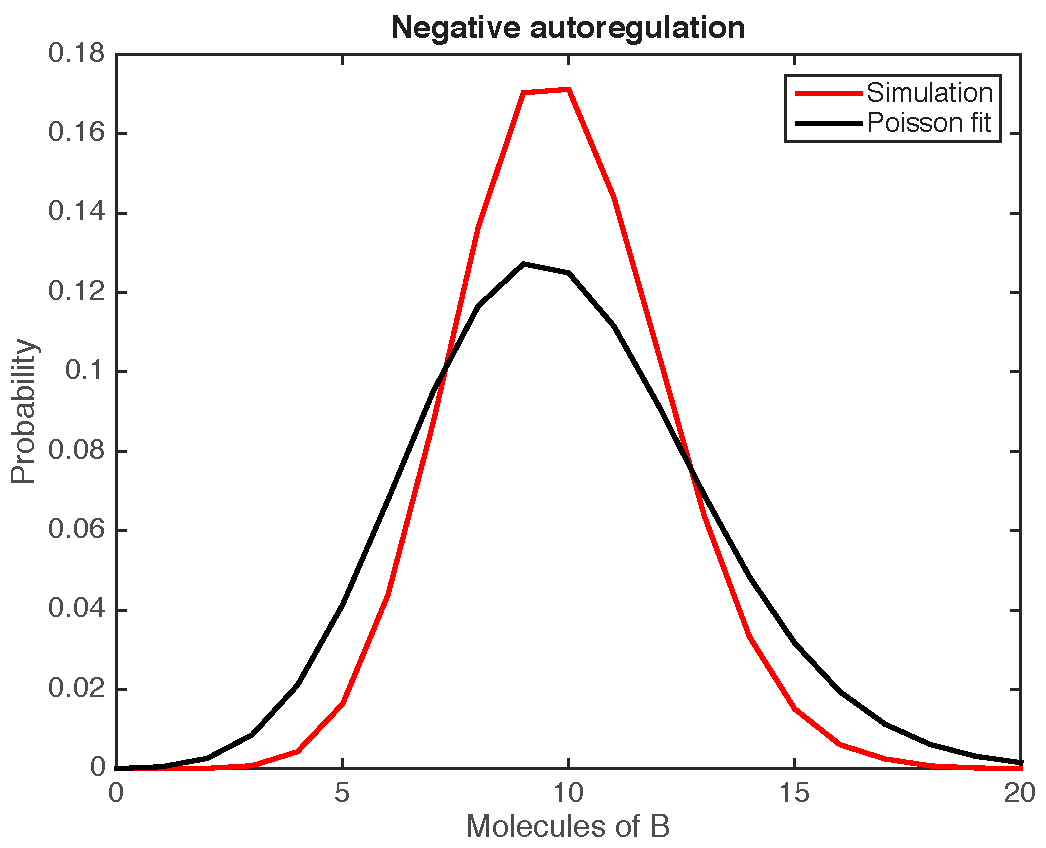
\includegraphics[width=0.4\textwidth]{prob1e.pdf}
\end{center}
{\color{red}
The simulation results for the negative autoregulation system have lower variance than the fitted Poisson distribution; this suggests that one use of negative regulation could be to limit variability.
}

\end{enumerate}

\end{document}